\documentclass[11pt,a4paper,reqno]{amsart}
\usepackage[utf8]{inputenc}
\usepackage[T1]{fontenc}
\usepackage[english]{babel}
\usepackage[osf]{mathpazo}
\usepackage{amsmath,amssymb}
\usepackage{mathtools}
\usepackage{microtype}
\usepackage[margin=3.1cm]{geometry}
\usepackage{graphicx}
\usepackage{float}
\usepackage{booktabs}
\usepackage{enumitem}
\usepackage{tikz}
\usetikzlibrary{shapes.geometric}
\usepackage[colorlinks=true,linkcolor=blue!45!black,citecolor=blue!45!black,urlcolor=blue!45!black]{hyperref}
\usepackage{xcolor}

\graphicspath{{../figures/}}
\linespread{1.06}

\newtheorem{theorem}{Theorem}[section]
\newtheorem{proposition}[theorem]{Proposition}
\newtheorem{lemma}[theorem]{Lemma}
\newtheorem{corollary}[theorem]{Corollary}
\theoremstyle{definition}
\newtheorem{definition}[theorem]{Definition}
\theoremstyle{remark}
\newtheorem{remark}[theorem]{Remark}

\newcommand{\PP}{\mathbb{P}}
\newcommand{\RR}{\mathbb{R}}
\newcommand{\ZZ}{\mathbb{Z}}
\newcommand{\Hex}{\mathrm{Hex}}
\newcommand{\Cor}{\mathrm{Cor}}
\newcommand{\Inn}{\mathrm{Inn}}
\newcommand{\Quad}{\mathrm{Quad}}
\newcommand{\Pent}{\mathrm{Pent}}
\DeclareMathOperator{\area}{area}
\newcommand{\shp}[1]{\tikz[baseline=-0.55ex]{\node[regular polygon,regular polygon sides=#1,draw,line width=0.5pt,minimum size=2.0ex,inner sep=0pt]{};}}
\newcommand{\gtri}{\shp{3}}
\newcommand{\gsq}{\shp{4}}
\newcommand{\gpent}{\shp{5}}
\newcommand{\ghex}{\shp{6}}

\title[A generalization of Marion Walter's theorem]{A One-Parameter Generalization\\ of Marion Walter's Theorem}
\author{D.~Berger}
\thanks{Prepared with assistance from Claude (Anthropic).}
\date{\today}

\begin{document}



\begin{abstract}\noindent
Marion Walter's theorem states that the central hexagon cut from a triangle by the six cevians joining each
vertex to the two \emph{trisection} points of the opposite side has area exactly $\tfrac{1}{10}$ of the triangle.
We replace the trisection points by the two points dividing each side in the ratios $t:1$ and $1:t$, obtaining a
one--parameter family. We set up the problem carefully in barycentric coordinates, define the discrete
(co)chain machinery used to compute areas, and \emph{derive} closed rational formulas in $t$ for the areas of all
five cell types ($6$ corner triangles, $6$ inner triangles, $3$ quadrilaterals, $3$ pentagons, $1$ hexagon),
proving that they tile the triangle. We then give three structural results: an incremental genealogy of the
subdivision; a proof that the combinatorial type is rigid for all $t>1$; and the arithmetic of the involution
$t\mapsto1/t$. The last point resolves a subtlety raised in discussion: the closed forms are \emph{signed}
(oriented) areas, and they are \emph{not} individually invariant under $t\mapsto1/t$; instead the corner triangles
grow into larger ``outer'' triangles while the quadrilaterals and pentagons reverse orientation, the signed total
remaining $1$. Passing to the invariant quotient coordinate $u=t+1/t$ exhibits the whole family as a degree--$2$
cover branched exactly at the median degeneration $t=1$, and splits each area into an invariant part and a
$\sqrt{u^2-4}$ part.
\end{abstract}

\maketitle

\tableofcontents

\section{Marion Walter's theorem}
Take a triangle and, on each side, mark the two points that cut it into three equal parts (the trisection
points). Join each vertex to the two trisection points of the \emph{opposite} side. The six segments so drawn are
\emph{cevians} --- segments from a vertex to the opposite side. They bound a small hexagon in the middle of the
triangle. Marion Walter's theorem (1993) asserts:
\begin{theorem}[Marion Walter]
The central hexagon has area equal to $\tfrac1{10}$ of the area of the triangle.
\end{theorem}
This is only a statement about \emph{one} of the regions produced. The six cevians in fact cut the triangle into
nineteen regions of several shapes; the hexagon is the innermost of them. The present note studies the whole
subdivision, and does so for a family of configurations indexed by a parameter $t$, of which Marion's is the case
$t=2$.

\begin{figure}[h]
\centering
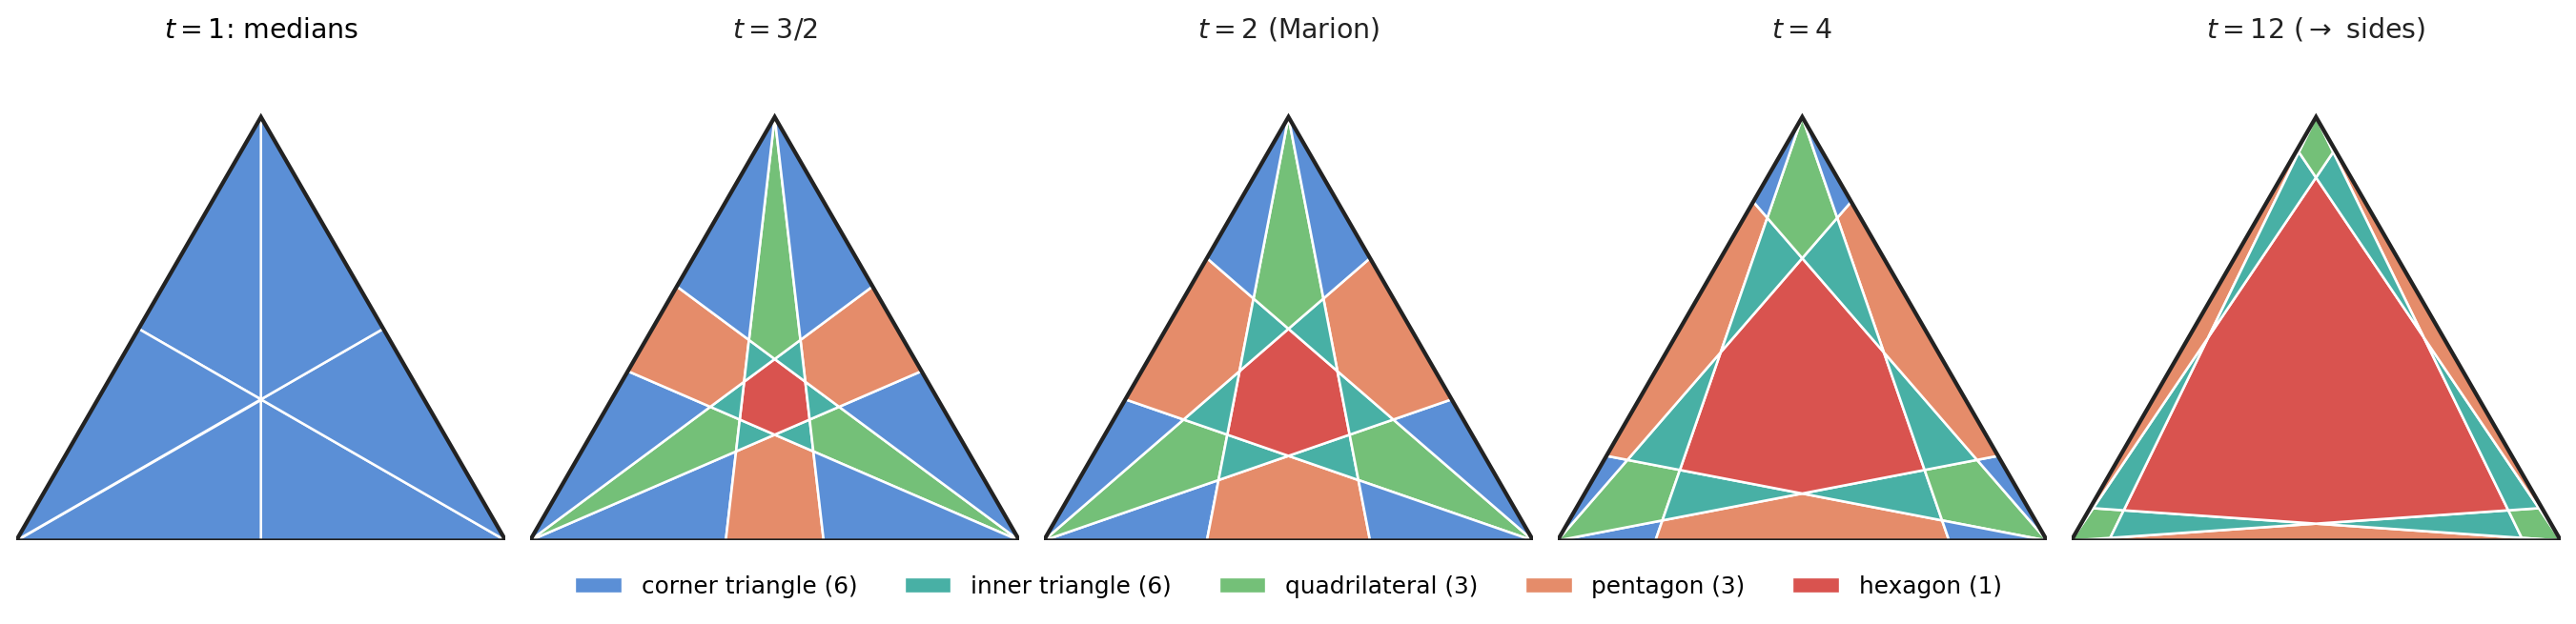
\includegraphics[width=\textwidth]{family_panels.png}
\caption{The family, with cells coloured by type. Far left: the degenerate case $t=1$, where the construction
collapses to the three medians and only six triangles remain. Middle: the generic (regular) type, the same for
every $t>1$, with Marion's configuration at $t=2$. Far right: as $t\to\infty$ the cevians fold onto the sides and
the hexagon fills the triangle.}
\label{fig:panels}
\end{figure}

\section{Setup and definitions}

\subsection{Barycentric coordinates}
Fix a triangle with vertices $A,B,C$.
\begin{definition}[Barycentric coordinates]
A point $P$ of the plane is written $P=(x:y:z)$ if $P=xA+yB+zC$ after normalising $x+y+z=1$; the triple is
determined up to a common nonzero scale, and we call it \emph{normalised} when $x+y+z=1$. The vertices are
$A=(1:0:0)$, $B=(0:1:0)$, $C=(0:0:1)$. The three sides are the loci
\[
BC:\ x=0,\qquad CA:\ y=0,\qquad AB:\ z=0 .
\]
A line is the zero set of a nonzero linear form $ax+by+cz$; we record it by its coefficient triple, the
\emph{covector} $\ell=[a:b:c]$ (itself defined only up to a common scale), and write $\ell\cdot P=ax+by+cz$ for the
incidence pairing. Points $[x:y:z]$ and lines $[a:b:c]$ are thus dual, and $P$ lies on $\ell$ exactly when
$\ell\cdot P=0$. In particular the three sides are $BC=[1:0:0]$, $CA=[0:1:0]$, $AB=[0:0:1]$.
\end{definition}
\begin{remark}[Correspondence with Cartesian coordinates]
Fix any Cartesian placement of the triangle, i.e.\ genuine position vectors $A,B,C\in\RR^2$ spanning a
non-degenerate triangle. A normalised barycentric point $(x,y,z)$ then sits at the Cartesian location
\[
P=xA+yB+zC=A+y\,(B-A)+z\,(C-A),\qquad x=1-y-z,
\]
so $(y,z)$ are ordinary affine coordinates with origin $A$ and basis $B-A,\ C-A$. Conversely a Cartesian point $P$
has barycentric coordinates equal to the signed area ratios $x=[P,B,C]$, $y=[A,P,C]$, $z=[A,B,P]$ (relative to
$ABC$), which sum to $1$. Substituting the parametrisation turns a barycentric line into an ordinary straight line:
\[
ax+by+cz=0\ \Longleftrightarrow\ a(1-y-z)+by+cz=0\ \Longleftrightarrow\ (b-a)\,y+(c-a)\,z+a=0,
\]
a genuine degree-one equation in $(y,z)$, and every Cartesian line arises this way. Hence the covector $[a:b:c]$ is
just the coefficient vector of a line, written symmetrically in the three barycentric variables; for example the
cevian $L_1:\,y=tz$ is $[\,0:1:-t\,]$.
\end{remark}
Barycentric coordinates are adapted to \emph{affine} geometry: any two triangles are related by an affine map,
and affine maps preserve ratios of areas. Hence every area \emph{ratio} computed below is the same for every
triangle, and we never need to fix the triangle's shape. The one fact we need is that areas are read off directly
from normalised coordinates:
\begin{lemma}[Barycentric area]\label{lem:area}
For points $P_i=(x_i:y_i:z_i)$, $i=1,2,3$, in normalised coordinates, the signed area of triangle $P_1P_2P_3$,
as a fraction of the area of $ABC$, equals the determinant
\[
[\,P_1,P_2,P_3\,]\;:=\;
\det\!\begin{pmatrix} x_1&y_1&z_1\\ x_2&y_2&z_2\\ x_3&y_3&z_3\end{pmatrix}.
\]
The sign is $+$ when $P_1P_2P_3$ is traversed counter-clockwise (the same orientation as $ABC$), and $-$
otherwise.
\end{lemma}
\begin{proof}
Use the last two coordinates as affine coordinates, $x_i=1-y_i-z_i$. Placing points in the plane by
$P=A+y\,(B-A)+z\,(C-A)$ identifies the $(y,z)$--plane with the plane affinely and sends $A,B,C$ to
$(y,z)=(0,0),(1,0),(0,1)$. An affine map multiplies every area by the same constant $\det[\,B-A,\ C-A\,]$, so
area \emph{ratios} may be computed directly in the $(y,z)$--plane. There $ABC$ has signed area $\tfrac12$ and
$P_1P_2P_3$ has signed area $\tfrac12\det\!\big[\begin{smallmatrix} y_2-y_1 & z_2-z_1\\ y_3-y_1 &
z_3-z_1\end{smallmatrix}\big]$, so their ratio is
\[
\frac{\text{signed area }P_1P_2P_3}{\text{area }ABC}
=\det\!\begin{pmatrix} y_2-y_1 & z_2-z_1\\ y_3-y_1 & z_3-z_1\end{pmatrix}.
\]
It remains to identify this with the $3\times3$ determinant. In $[\,P_1,P_2,P_3\,]$ replace the first column by
the sum of all three columns; since $x_i+y_i+z_i=1$ that column becomes all ones, so
$[\,P_1,P_2,P_3\,]=\det\!\big[\begin{smallmatrix} 1&y_1&z_1\\ 1&y_2&z_2\\ 1&y_3&z_3\end{smallmatrix}\big]$.
Subtracting the first row from the other two and expanding along the first column returns exactly the $2\times2$
determinant above. Finally, with $A,B,C$ labelled counter-clockwise the embedding preserves orientation, so the
determinant is positive precisely when $P_1P_2P_3$ runs counter-clockwise.
\end{proof}
For instance, with the centroid $G=(\tfrac13:\tfrac13:\tfrac13)$ one checks $[G,A,B]=[G,B,C]=[G,C,A]=\tfrac13$,
and their sum is $1$: the three triangles $GAB,GBC,GCA$ tile $ABC$.

\subsection{The cevian lines}
On side $BC$ place the two points dividing it in the ratios $t:1$ and $1:t$, i.e.\ the points
$(0:t:1)$ and $(0:1:t)$; at $t=2$ these are the trisection points $(0:2:1),(0:1:2)$. The cevian from $A=(1:0:0)$
through $(0:t:1)$ is the line $\{\,y=tz\,\}$, and through $(0:1:t)$ the line $\{\,z=ty\,\}$. Cycling
$A\to B\to C$ (that is $x\to y\to z\to x$) gives all six:
\[
\begin{array}{lll}
L_1:\ y=tz, & L_2:\ z=ty & \text{(from $A$)},\\
L_3:\ z=tx, & L_4:\ x=tz & \text{(from $B$)},\\
L_5:\ x=ty, & L_6:\ y=tx & \text{(from $C$)}.
\end{array}
\]
The classical Marion configuration is $t=2$.

\subsection{Chains, cochains and the coboundary}
The six cevians and the three sides cut the triangle into vertices, edges and cells; this is a finite
\emph{CW--complex} $X$ (a space built from $0$--cells = points, $1$--cells = edges, $2$--cells = polygonal
regions). We compute areas with the standard discrete apparatus, which we now define from scratch.

\begin{definition}[Chains]
Orient every edge and every cell. For $k=0,1,2$ the group $C_k(X)$ of \emph{$k$--chains} is the set of formal
$\RR$--linear combinations of the (oriented) $k$--cells. The \emph{boundary operator}
$\partial\colon C_k\to C_{k-1}$ sends a cell to the signed sum of the cells on its boundary; concretely, the
boundary of an oriented polygonal cell is the cycle of its edges, each taken with $+$ if its orientation agrees
with the boundary traversal and $-$ otherwise.
\end{definition}

\begin{definition}[Cochains and coboundary]
A \emph{$k$--cochain} is a linear functional on $k$--chains, i.e.\ an element of $C^k(X):=\operatorname{Hom}(C_k(X),\RR)$;
equivalently, a rule assigning a real number to each oriented $k$--cell (a $1$--cochain assigns numbers to edges, a
$2$--cochain assigns numbers to cells). The \emph{coboundary operator}
\[
\delta\colon C^{k}(X)\longrightarrow C^{k+1}(X),\qquad (\delta\varphi)(\sigma):=\varphi(\partial\sigma),
\]
is the transpose of $\partial$: to evaluate $\delta\varphi$ on a cell, evaluate $\varphi$ on that cell's boundary
cycle of edges.
\end{definition}

\begin{proposition}[Area is a coboundary]\label{prop:cob}
Fix a basepoint $O$ and define the $1$--cochain
\[
\alpha([P,Q]) \;=\; [\,O,P,Q\,]
\]
(the signed area ratio of triangle $OPQ$, Lemma~\ref{lem:area}). Then the \emph{area $2$--cochain} $\mathcal A$,
which assigns to each cell its signed area ratio, satisfies
\[
\mathcal A \;=\; \delta\alpha .
\]
That is, the signed area of a cell equals $\sum_{[P,Q]\in\partial(\text{cell})}[\,O,P,Q\,]$.
\end{proposition}
\begin{proof}
Triangulate the cell by joining $O$ to each boundary edge; the triangles $OPQ$ fill the cell, and the internal
spokes $OP$ appear twice with opposite orientation and cancel (a telescoping sum). What remains is the sum over
boundary edges, which is exactly $(\delta\alpha)(\text{cell})$. This is the shoelace formula, read as the discrete
Stokes theorem ``$\int_{\text{cell}}dA=\oint_{\partial}\alpha$''.
\end{proof}
Two consequences: changing $O$ replaces $\alpha$ by $\alpha+\delta f$ for a $0$--cochain $f$, so
$\mathcal A=\delta\alpha$ is unchanged (gauge invariance); and, being a coboundary, the area of a cell depends only
on its boundary cycle. We take $O=G$, the centroid, throughout. \emph{Orientation matters}: a cell traversed
clockwise gets a negative signed area. We will keep the signs; they are the crux of Section~\ref{sec:galois}.

\section{Explicit computation of the cell areas}\label{sec:areas}
Every cell vertex is an intersection of two of the nine lines, computed by solving the two linear forms. We
carry out two representative cases in full; the rest are identical in spirit.

\subsection{A corner triangle}
Consider the small triangle at vertex $A$ bounded by the side $AB$ and by the cevians $L_5$ and $L_1$. Its three
vertices are
\[
A=(1:0:0),\qquad
AB\cap L_5=\Big(\tfrac{t}{t+1}:\tfrac{1}{t+1}:0\Big),\qquad
L_5\cap L_1=\Big(\tfrac{t^2}{D}:\tfrac{t}{D}:\tfrac1D\Big),\quad D:=t^2+t+1,
\]
where $AB\cap L_5$ solves $z=0,\ x=ty$, and $L_5\cap L_1$ solves $x=ty,\ y=tz$. By Lemma~\ref{lem:area},
\[
\Cor(t)=\det\!\begin{pmatrix}
1&0&0\\[2pt]
\tfrac{t}{t+1}&\tfrac{1}{t+1}&0\\[2pt]
\tfrac{t^2}{D}&\tfrac{t}{D}&\tfrac1D
\end{pmatrix}
=1\cdot\Big(\tfrac{1}{t+1}\cdot\tfrac1D-0\Big)
=\frac{1}{(t+1)(t^2+t+1)} .
\]

\subsection{The hexagon}
The hexagon is bounded by all six cevians; its vertices are the six ``inner'' intersections
\[
\begin{aligned}
&L_1\cap L_4=\tfrac{(t:t:1)}{2t+1},\ &&L_4\cap L_5=\tfrac{(t:1:1)}{t+2},\ &&L_5\cap L_2=\tfrac{(t:1:t)}{2t+1},\\
&L_2\cap L_3=\tfrac{(1:1:t)}{t+2},\ &&L_3\cap L_6=\tfrac{(1:t:t)}{2t+1},\ &&L_6\cap L_1=\tfrac{(1:t:1)}{t+2}.
\end{aligned}
\]
Fanning from the centroid $G$ (Proposition~\ref{prop:cob}) and summing the six determinants
$[\,G,v_i,v_{i+1}\,]$ gives, after simplification,
\[
\Hex(t)=\frac{2(t-1)^2}{(t+2)(2t+1)} .
\]
(The three--fold symmetry collapses the six determinants into two equal orbits of three, so only two distinct
determinants must be evaluated.)

\subsection{The five formulas}
Carrying out the same computation for the remaining classes yields, as fractions of the triangle's area:
\begin{align}
\Hex(t)&=\frac{2(t-1)^2}{(t+2)(2t+1)}, & &\text{(hexagon, $\times1$)}\label{e:hex}\\[3pt]
\Inn(t)&=\frac{t\,(t-1)^2}{(t+2)(2t+1)(t^2+t+1)}, & &\text{(inner triangle, $\times6$)}\label{e:inn}\\[3pt]
\Cor(t)&=\frac{1}{(t+1)(t^2+t+1)}, & &\text{(corner triangle, $\times6$)}\label{e:cor}\\[3pt]
\Quad(t)&=\frac{2(t-1)}{(t+2)(t^2+t+1)}, & &\text{(quadrilateral, $\times3$)}\label{e:quad}\\[3pt]
\Pent(t)&=\frac{(t-1)(t^2+3t+1)}{(t+1)(2t+1)(t^2+t+1)}. & &\text{(pentagon, $\times3$)}\label{e:pent}
\end{align}

\begin{proposition}[Tiling identity]\label{prop:tile}
$\Hex+6\,\Inn+6\,\Cor+3\,\Quad+3\,\Pent=1$ identically in $t$.
\end{proposition}
\begin{proof}
Over the common denominator $(t+1)(t+2)(2t+1)(t^2+t+1)$ the five numerators sum to
\[
2t^5+9t^4+16t^3+16t^2+9t+2,
\]
which is precisely that denominator expanded. Hence the sum is $1$.
\end{proof}

\noindent\textbf{Marion, $t=2$.} Substituting $t=2$ into \eqref{e:hex}--\eqref{e:pent}:
\[
\Hex=\tfrac1{10},\quad \Inn=\tfrac1{70},\quad \Cor=\tfrac1{21},\quad \Quad=\tfrac1{14},\quad \Pent=\tfrac{11}{105},
\]
and $\tfrac1{10}+6\cdot\tfrac1{70}+6\cdot\tfrac1{21}+3\cdot\tfrac1{14}+3\cdot\tfrac{11}{105}
=\tfrac{21+18+60+45+66}{210}=1$, recovering Marion's $\tfrac1{10}$. Note each pentagon,
$\tfrac{11}{105}\approx0.10476$, is slightly \emph{larger} than the hexagon $0.1$, by $\tfrac1{210}$.

\begin{figure}[h]
\centering
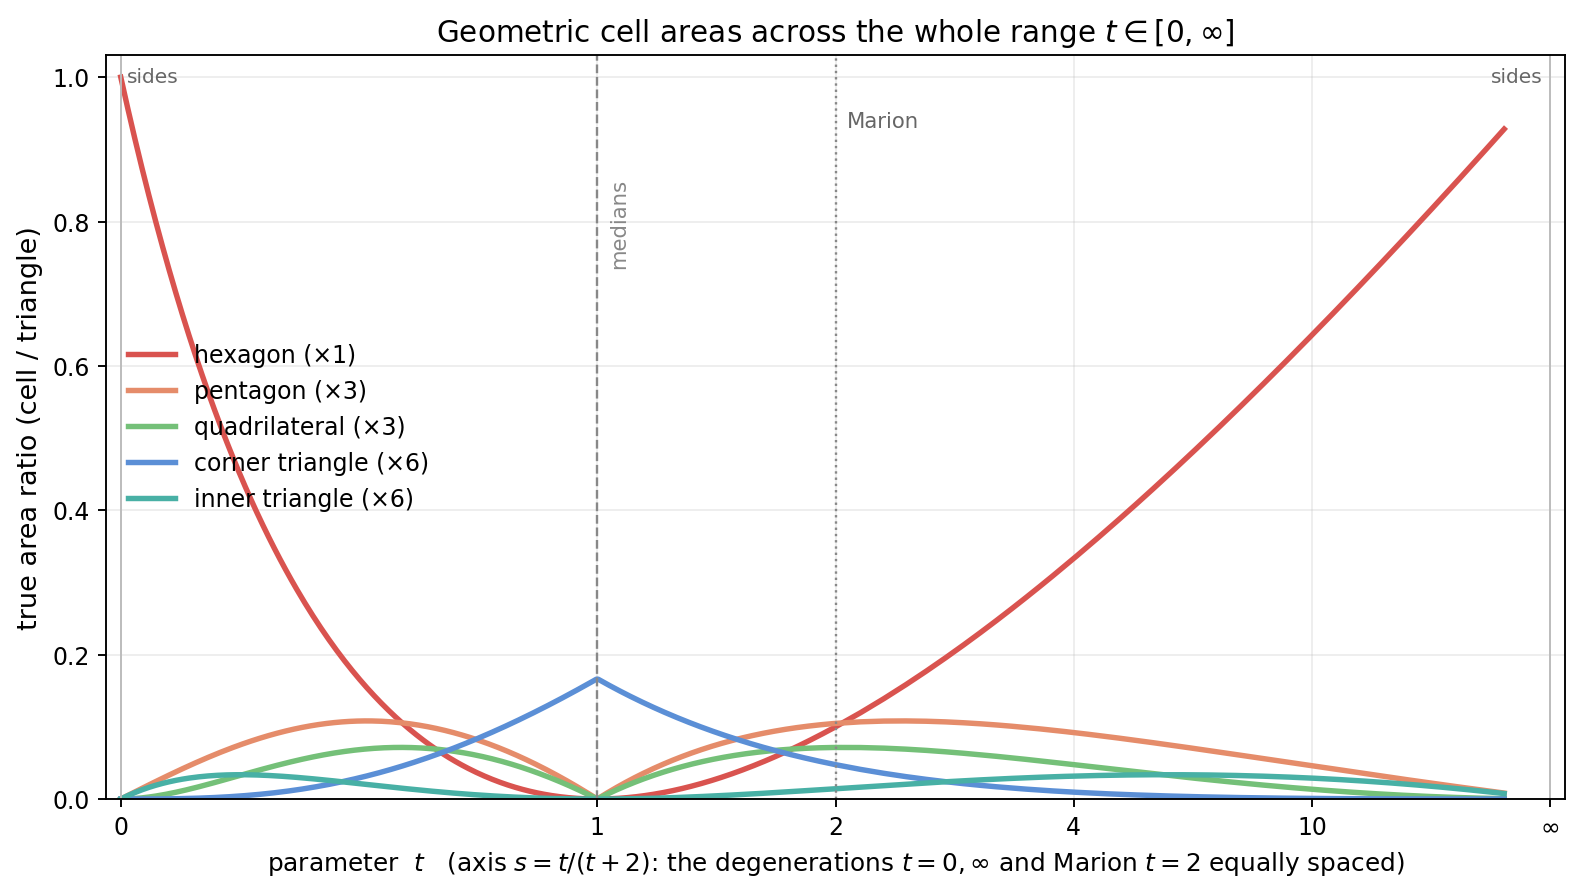
\includegraphics[width=0.92\textwidth]{cell_areas.png}
\caption{The five true (unsigned) area ratios across the whole range. The horizontal axis is reparametrised by
$s=t/(t+2)$, so that the two degenerations $t=0$ and $t=\infty$ and the Marion point $t=2$ sit at equal spacing
$s=0,\tfrac12,1$. For $t<1$ the true areas are the mirror images of $t>1$ under $t\mapsto1/t$ (Section
\ref{sec:galois}).}
\label{fig:areas}
\end{figure}

\subsection{Degenerations and the three cases}
\begin{enumerate}[leftmargin=1.7em]
\item \textbf{Regular} ($t\neq0,1,\infty$): census $12/3/3/1$. As shown in Section~\ref{sec:rigid} this single
combinatorial type persists for all $t>1$ (and, mirrored, for $0<t<1$); Marion $t=2$ is its representative.
\item \textbf{Median} $t=1$: the two feet on each side merge, the six cevians become the three medians, and only
$6$ triangles survive (each $\tfrac16$). Every formula except $\Cor$ carries a factor $(t-1)$ and vanishes.
\item \textbf{Sides} $t=0$ or $t\to\infty$: the feet reach the vertices, the cevians lie along the sides, and the
hexagon fills the triangle ($\Hex\to1$).
\end{enumerate}

\section{The incremental construction (genealogy of the subdivision)}
Draw the cevians one at a time, in the order $A_1,A_2$ (the two from $A$), then $B_1,B_2$, then $C_1,C_2$. A
straight chord meets a convex cell in a single segment and so splits it into exactly two pieces. Recording, for
each new piece, which old cell it came from produces a binary \emph{genealogy tree}: one triangle at the root,
nineteen cells at the leaves (Figure~\ref{fig:tree}).

The two cevians from $A$ fan the triangle into three triangles. Adding $B_1$ then cuts across that fan: it enters
the triangle at the vertex $B$ (splitting one fan--triangle into two triangles), and passes through the other two
fan--triangles, cutting each into a triangle and a \emph{quadrilateral}. Thus already at the step $+B_1$ two
quadrilaterals appear; the running census becomes $4$ triangles and $2$ quadrilaterals. The productions of the
whole process are governed by the following splitting law.

\emph{The general splitting law.} A chord across a convex $m$--gon meets the boundary in two points $P,Q$; let
$\nu\in\{0,1,2\}$ be the number of these that are \emph{vertices} of the $m$--gon (the others lying in edge
interiors). The points $P,Q$ cut the boundary into two arcs carrying $a$ and $b$ of the \emph{remaining}
vertices, with $a+b=m-\nu$. Both $P$ and $Q$ are corners of both pieces, so the pieces are an $(a+2)$--gon and a
$(b+2)$--gon, with side--sum
\[
(a+2)+(b+2)=m+4-\nu .
\]
The split therefore depends on how the chord meets the boundary:
\begin{itemize}[leftmargin=1.7em,itemsep=1pt]
\item $\nu=0$ (general position, through no vertex): side--sum $m+4$; slicing off a single corner ($a=1$) gives
$\gtri+\big((m{+}1)\text{--gon}\big)$, e.g.\ $\gtri\to\gtri+\gsq$, $\gsq\to\gtri+\gpent$, $\gpent\to\gtri+\ghex$;
\item $\nu=1$ (through exactly one vertex): side--sum $m+3$; e.g.\ a triangle cut from a vertex to the opposite
edge has $a=b=1$, giving $\gtri\to\gtri+\gtri$;
\item $\nu=2$ (a diagonal, through two vertices): side--sum $m+2$; e.g.\ a diagonal of a quadrilateral gives
$\gsq\to\gtri+\gtri$, of a pentagon $\gpent\to\gtri+\gsq$.
\end{itemize}
So the productions are \emph{not} automatic --- they hold only when the chord avoids vertices. In the Marion
construction general position is guaranteed for $t>1$ by the rigidity of Section~\ref{sec:rigid}: no three of the
six cevians are concurrent, so a new cevian never runs through an interior cell vertex (that would be a triple
point). Hence every interior cut is in general position ($\nu=0$), and one checks stage by stage that it slices a
single corner ($a=1$); the only $\nu=1$ event is a cevian issuing from \emph{its own} triangle vertex (which
splits the corner cell $\gtri\to\gtri+\gtri$), and the diagonal case $\nu=2$ never occurs. This yields exactly the
four realized productions
\[
\gtri\to\gtri+\gtri,\qquad \gtri\to\gtri+\gsq,\qquad \gsq\to\gtri+\gpent,\qquad \gpent\to\gtri+\ghex ,
\]
each cut shaving off a triangle and lifting one neighbour by a side. Because a hexagon needs all six cevians on
its boundary, it can be produced only by the sixth and last cevian --- and there is exactly one.

\begin{figure}[h]
\centering
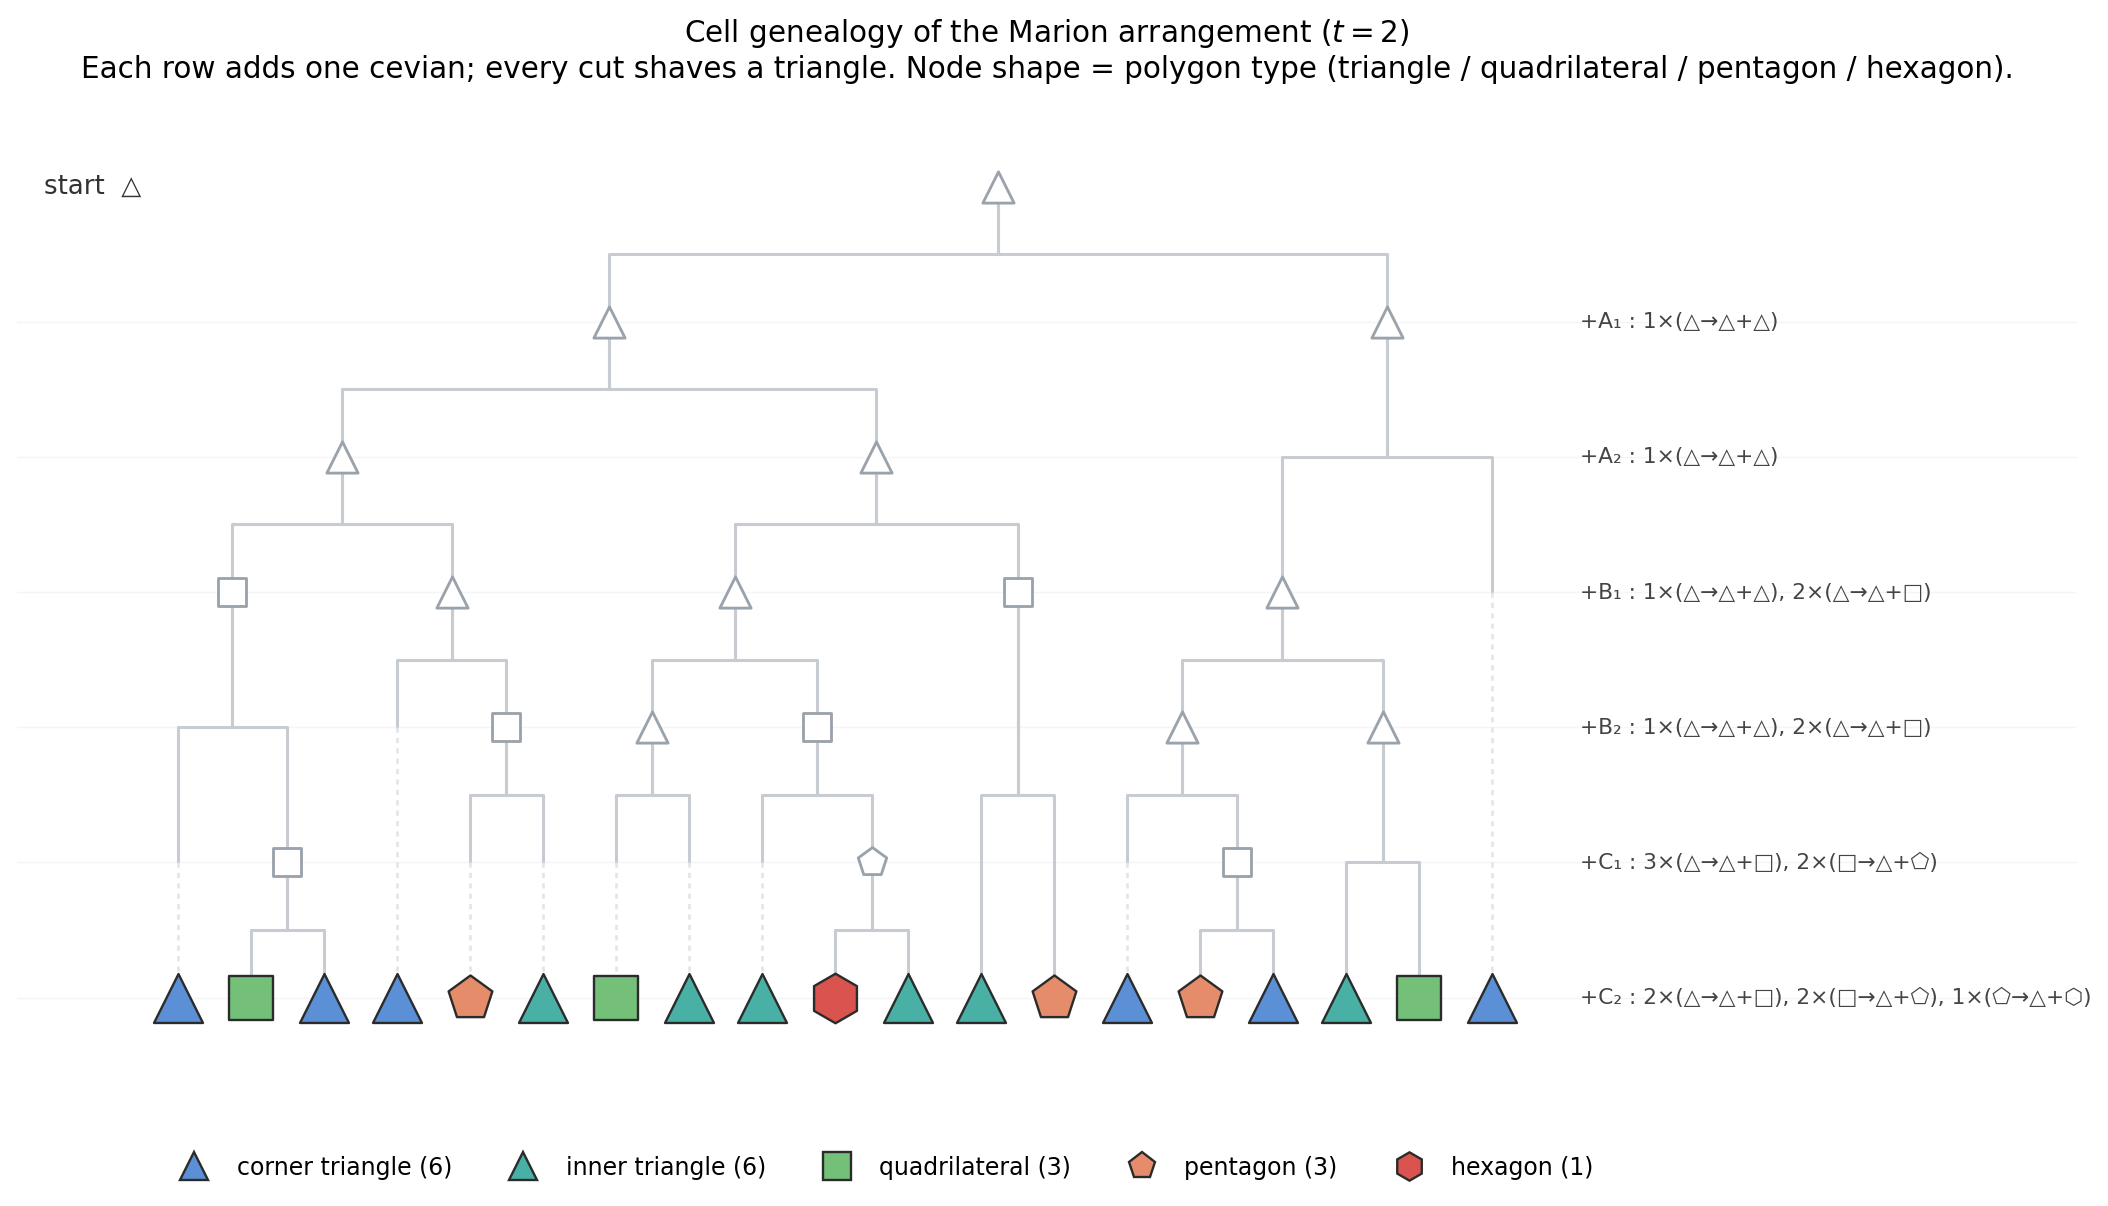
\includegraphics[width=\textwidth]{genealogy_tree.png}
\caption{The genealogy for $t=2$. Each row adds one cevian; each fork is one chord splitting one cell. Each node
is drawn as its polygon (triangle / quadrilateral / pentagon / hexagon); leaves (aligned at the bottom) are
coloured by final type. The split rules per stage are listed on the right. The hexagon is born only at the very
last cut.}
\label{fig:tree}
\end{figure}

\subsection{Why exactly these types: the boundary signature}
Label each final cell by the pair (number of triangle sides, number of cevians) on its boundary. The polygon
degree is their sum, so the census is forced:
\begin{center}
\begin{tabular}{lccc}
\toprule
cell type & triangle sides & cevians & count \\
\midrule
corner triangle & $1$ & $2$ & $6$\\
inner triangle  & $0$ & $3$ & $6$\\
quadrilateral   & $0$ & $4$ & $3$\\
pentagon        & $1$ & $4$ & $3$\\
hexagon         & $0$ & $6$ & $1$\\
\bottomrule
\end{tabular}
\end{center}
A hexagon needs all six cevians, so it is unique and central; the multiplicities $6{+}6/3/3/1$ are the orbit
sizes of the three--fold rotational symmetry.

\subsection{Rigidity for $t>1$}\label{sec:rigid}
\begin{definition}[Concurrence, concurrence determinant]
Three distinct lines are \emph{concurrent} if they pass through one common point. In barycentric coordinates a
line is a covector $\ell=[a:b:c]$ acting by the incidence $ax+by+cz=0$, and a point $P=[x:y:z]$ lies on $\ell$ iff
$\ell\cdot P=0$. A point lies on all of $\ell_1,\ell_2,\ell_3$ iff the homogeneous system with coefficient matrix
\[
M=\begin{pmatrix} a_1&b_1&c_1\\ a_2&b_2&c_2\\ a_3&b_3&c_3\end{pmatrix}
\]
has a nonzero solution $P$. Hence the three lines are concurrent \emph{iff} the \emph{concurrence determinant}
$\det M$ vanishes. (Dually: three lines are concurrent iff their covectors are linearly dependent.)

An arrangement of lines is in \emph{general position} when no three of them are concurrent --- equivalently, when
every intersection point lies on exactly two lines. It suffices to test \emph{triples}: two lines already meet in
a single point, so the first possible degeneracy is a triple point, and any point common to $k\ge3$ lines contains
three concurrent lines among them. Ruling out all concurrent triples therefore rules out every higher multiple
point at once.
\end{definition}

Written as covectors, the six cevians are
\[
\begin{array}{lll}
L_1=[0:1:-t], & L_2=[0:-t:1] & \text{(from $A$)},\\
L_3=[-t:0:1], & L_4=[1:0:-t] & \text{(from $B$)},\\
L_5=[1:-t:0], & L_6=[-t:1:0] & \text{(from $C$)}.
\end{array}
\]

\begin{lemma}\label{lem:transversal}
For $t\neq0$, only \emph{transversal} triples --- one cevian from each vertex --- can be concurrent.
\end{lemma}
\begin{proof}
The two cevians issuing from a common vertex, say $L_1,L_2$ from $A$, meet only at $A=[1:0:0]$. A third cevian is
concurrent with them iff it also passes through $A$, i.e.\ iff its covector $[a:b:c]$ satisfies $a=0$. But
$L_3,\dots,L_6$ all have $a=\pm t\neq0$ or $a=1$; none passes through $A$. The same holds at $B,C$. So a triple
containing two cevians from one vertex is never concurrent, leaving only the $2\cdot2\cdot2=8$ transversal triples.
\end{proof}

\begin{proposition}\label{prop:rigid}
Each transversal triple has concurrence determinant $\pm(t-1)(t^2+t+1)$ or $\pm\,t(t-1)$; since $t^2+t+1>0$ for
all real $t$, the only positive root is $t=1$. Consequently, for every $t>1$ no three cevians are concurrent: the
six lines are in general position, and the whole combinatorial arrangement --- genealogy tree and census
$12/3/3/1$ alike --- is constant on $(1,\infty)$, with only the areas varying.
\end{proposition}
\begin{proof}
Evaluate $\det M$ on all eight transversal triples. The two \emph{cyclic} triples give, for instance,
\[
\det\!\begin{pmatrix}0&1&-t\\ -t&0&1\\ 1&-t&0\end{pmatrix}
=-1\,(-t\cdot0-1\cdot1)+(-t)\,\big((-t)(-t)-0\big)=1-t^3=-(t-1)(t^2+t+1),
\]
and likewise $\{L_2,L_4,L_6\}$ gives $-(t-1)(t^2+t+1)$. Each of the remaining six triples gives, e.g.
\[
\det\!\begin{pmatrix}0&1&-t\\ -t&0&1\\ -t&1&0\end{pmatrix}
=-1\,(0+t)+(-t)(-t)=t^2-t=t(t-1),
\]
so $\{L_1,L_3,L_6\},\{L_1,L_4,L_5\},\{L_1,L_4,L_6\},\{L_2,L_3,L_5\},\{L_2,L_3,L_6\},\{L_2,L_4,L_5\}$ all give
$t(t-1)$. The quadratic $t^2+t+1$ has discriminant $-3<0$, hence is strictly positive; therefore
$(t-1)(t^2+t+1)=0$ only at $t=1$, and $t(t-1)=0$ only at $t=0$ or $t=1$. For $t>1$ every one of the eight
determinants is nonzero, so no transversal triple is concurrent; with Lemma~\ref{lem:transversal} this means no
three of the six cevians meet at a point. General position of the six lines fixes all incidences among them, so
the face lattice --- and with it the genealogy and the census $12/3/3/1$ --- cannot change as $t$ varies over
$(1,\infty)$; only the vertex positions, and hence the areas, move.
\end{proof}

\begin{remark}
At $t=1$ all eight determinants vanish simultaneously: every transversal triple is concurrent and the six cevians
collapse onto the three medians (concurrent at the centroid). This is the unique value $t>0$ at which the type
degenerates; at $t=0$ only the six $t(t-1)$ triples vanish, matching the ``sides'' degeneration. By the involution
$t\mapsto1/t$ the mirror range $0<t<1$ carries the same combinatorial type as $(1,\infty)$.
\end{remark}

\section{The involution $t\mapsto1/t$: orientation and Galois structure}\label{sec:galois}
Each area \eqref{e:hex}--\eqref{e:pent} is a rational function of $t$, hence a morphism $\PP^1_t\to\PP^1$ of
projective lines (the values $t=0,1,\infty$ are genuine points of the domain, not gaps). The projective line, not
the affine line, is the correct parameter space.

\subsection{The picture is invariant; the signed formulas are not}
The configuration depends only on the \emph{unordered} pair of feet on each side, so replacing $t$ by $1/t$
(which swaps the two feet, hence swaps the two cevians $L_1\leftrightarrow L_2$, etc.) leaves the six lines
\emph{as a set} unchanged. Consequently the nineteen cells, and the multiset of their true (unsigned) areas, are
literally the same at $t$ and $1/t$. In this sense the involution induces a $\ZZ/2$ action permuting the cells of
each type among themselves, and the \emph{unsigned} areas are invariant.

The closed forms \eqref{e:hex}--\eqref{e:pent}, however, are \emph{signed} areas attached to a specific
orientation and to a $t$--dependent labelling of the cevians. They are \emph{not} individually invariant. Indeed,
evaluating the signed formulas at $t=2$ and at its mirror $t=\tfrac12$:
\begin{center}
\begin{tabular}{lccccc}
\toprule
& hexagon & inner $\times6$ & corner $\times6$ & quad $\times3$ & pent $\times3$ \\
\midrule
$t=2$   & $\tfrac1{10}$ & $\tfrac{3}{35}$ & $\tfrac{2}{7}$ & $\tfrac{3}{14}$ & $\tfrac{11}{35}$ \\[2pt]
$t=1/2$ & $\tfrac1{10}$ & $\tfrac{3}{35}$ & $\tfrac{16}{7}$ & $-\tfrac{24}{35}$ & $-\tfrac{11}{14}$ \\
\bottomrule
\end{tabular}
\end{center}
Both rows sum to $1$ (Proposition~\ref{prop:tile} holds identically), but the individual entries differ wildly.
The resolution is exactly the orientation bookkeeping suggested by the shape change across the branch point
$t=1$: the corner--triangle \emph{construction} (vertices $A,\ AB\cap L_5,\ L_5\cap L_1$) yields a small interior
triangle for $t>1$ but a much larger ``outer'' triangle for $t<1$ (its area grows from $\tfrac1{21}$ to
$\tfrac{8}{21}$), while the quadrilaterals and pentagons \emph{reverse orientation} and so contribute with a minus
sign. The overcount by the enlarged corner triangles is cancelled exactly by the now--negative
quadrilaterals and pentagons, and the signed total returns to $1$ (Figures~\ref{fig:orient},~\ref{fig:signed},~\ref{fig:move}). Figure~\ref{fig:move}
tracks all five types at once.
The true geometric area of each actual cell is recovered as the value on the sheet $t\ge1$ (equivalently as an
absolute value), and is invariant --- consistent with the picture being fixed.

\begin{figure}[H]
\centering
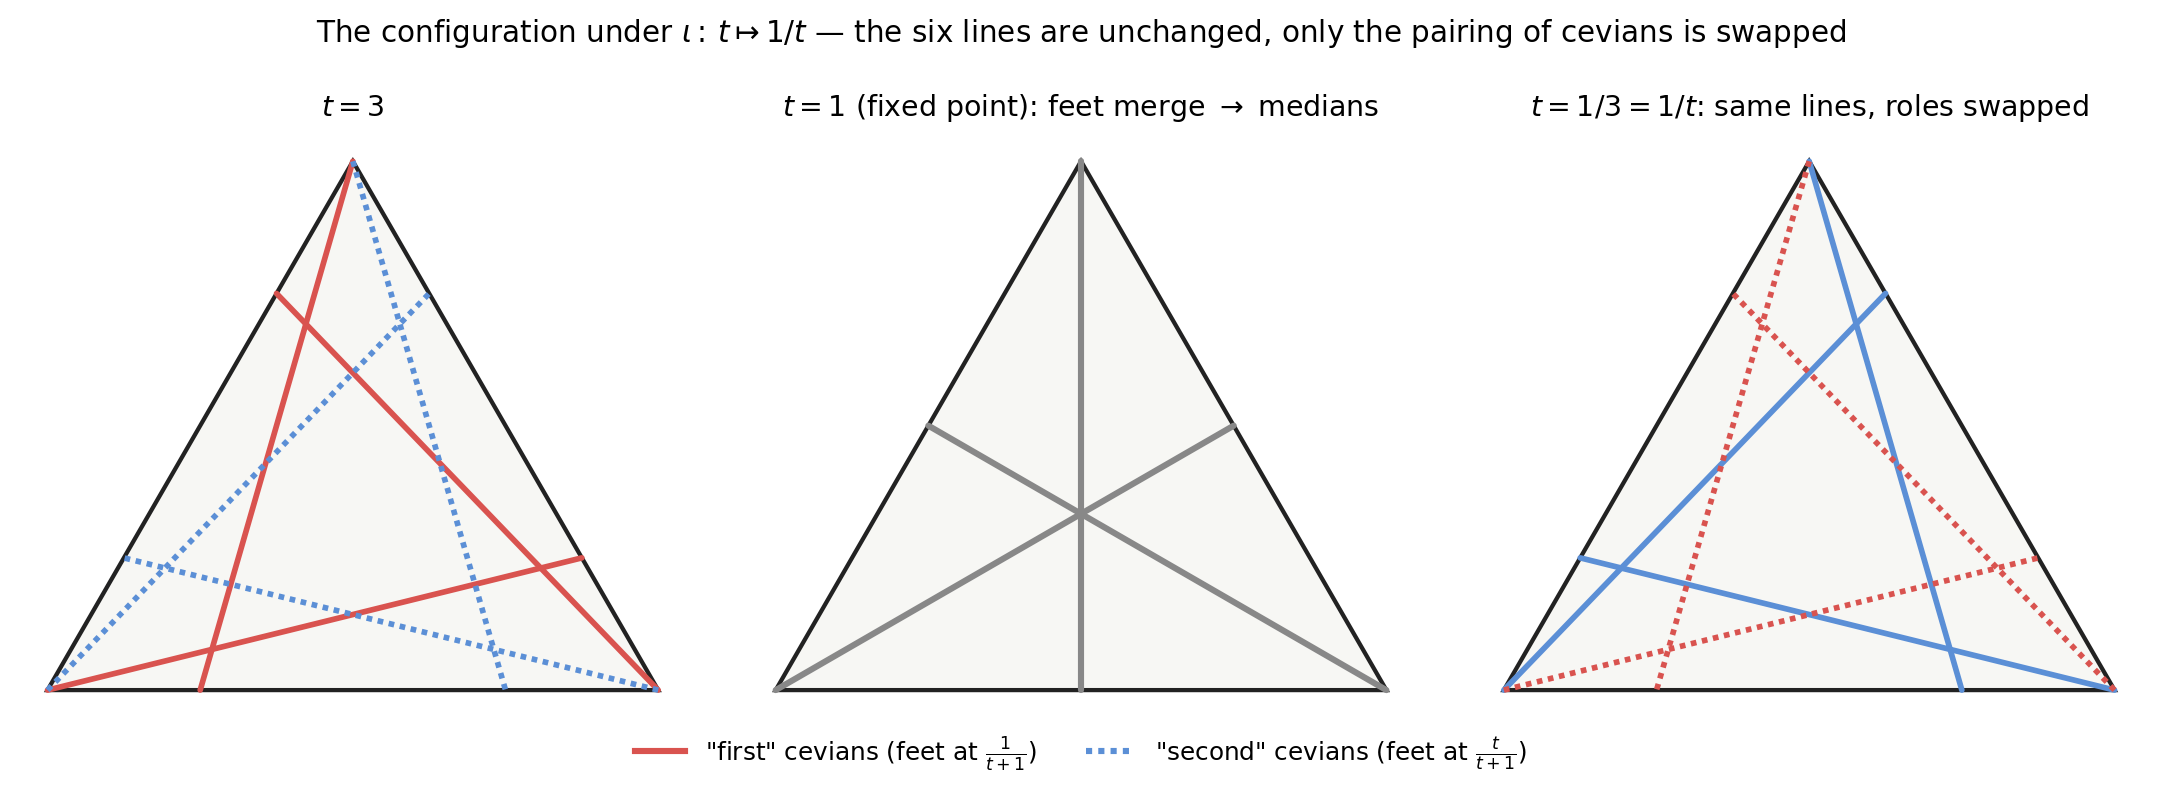
\includegraphics[width=0.62\textwidth]{involution_cevians.png}
\caption{The involution on the cevians. The outer two panels ($t=3$ and $t=1/3=1/t$) are the \emph{same} six
lines; only the roles of the paired cevians (solid/dotted) are exchanged. At the fixed point $t=1$ the paired
feet merge and the cevians become the three medians.}
\label{fig:involution}
\end{figure}

\begin{figure}[H]
\centering
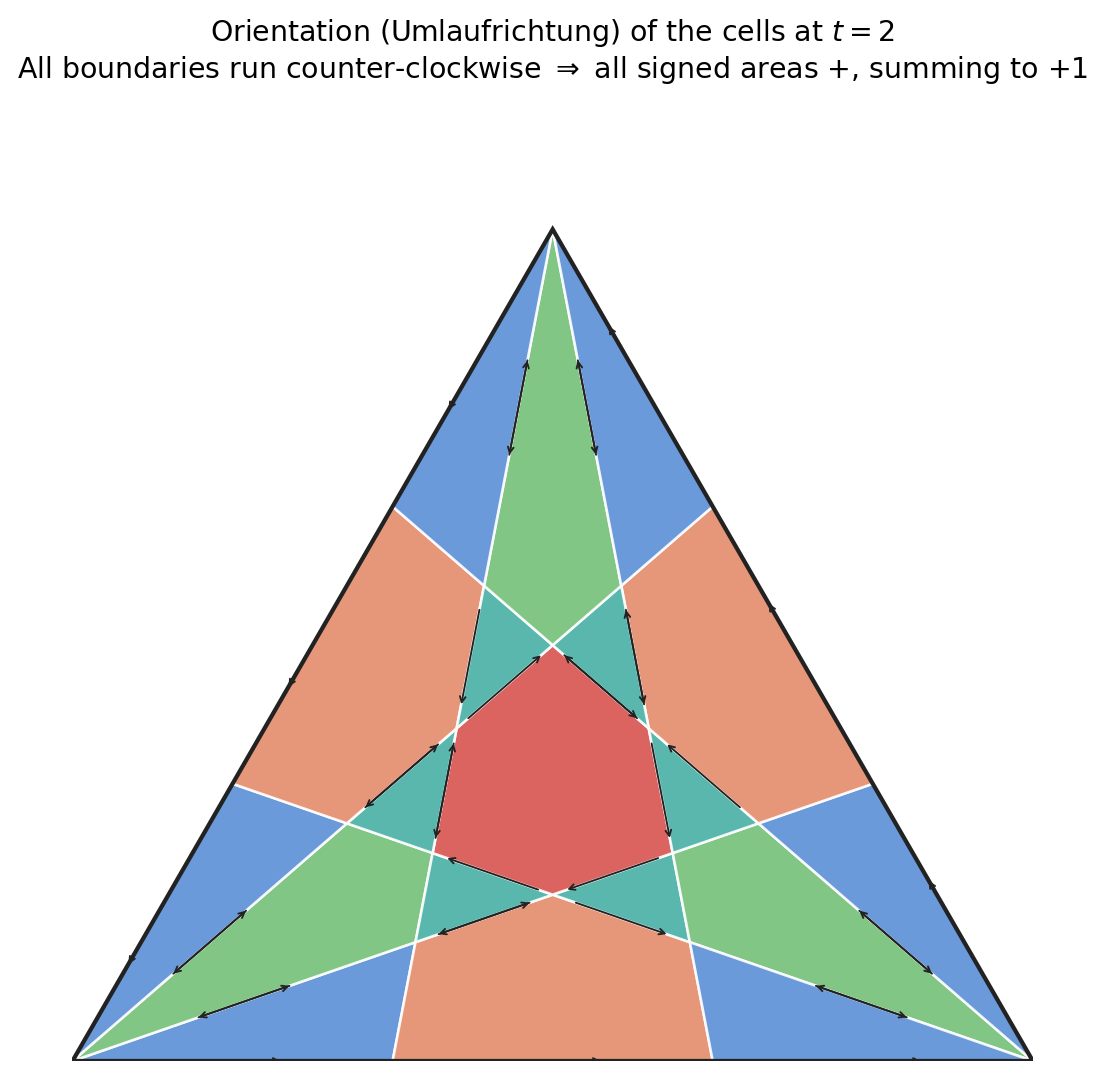
\includegraphics[width=0.60\textwidth]{orientation.png}
\caption{Orientation of the cells at $t=2$: every boundary is traversed counter-clockwise, so every signed area is
positive and the signed total is $+1$.}
\label{fig:orient}
\end{figure}

\begin{figure}[H]
\centering
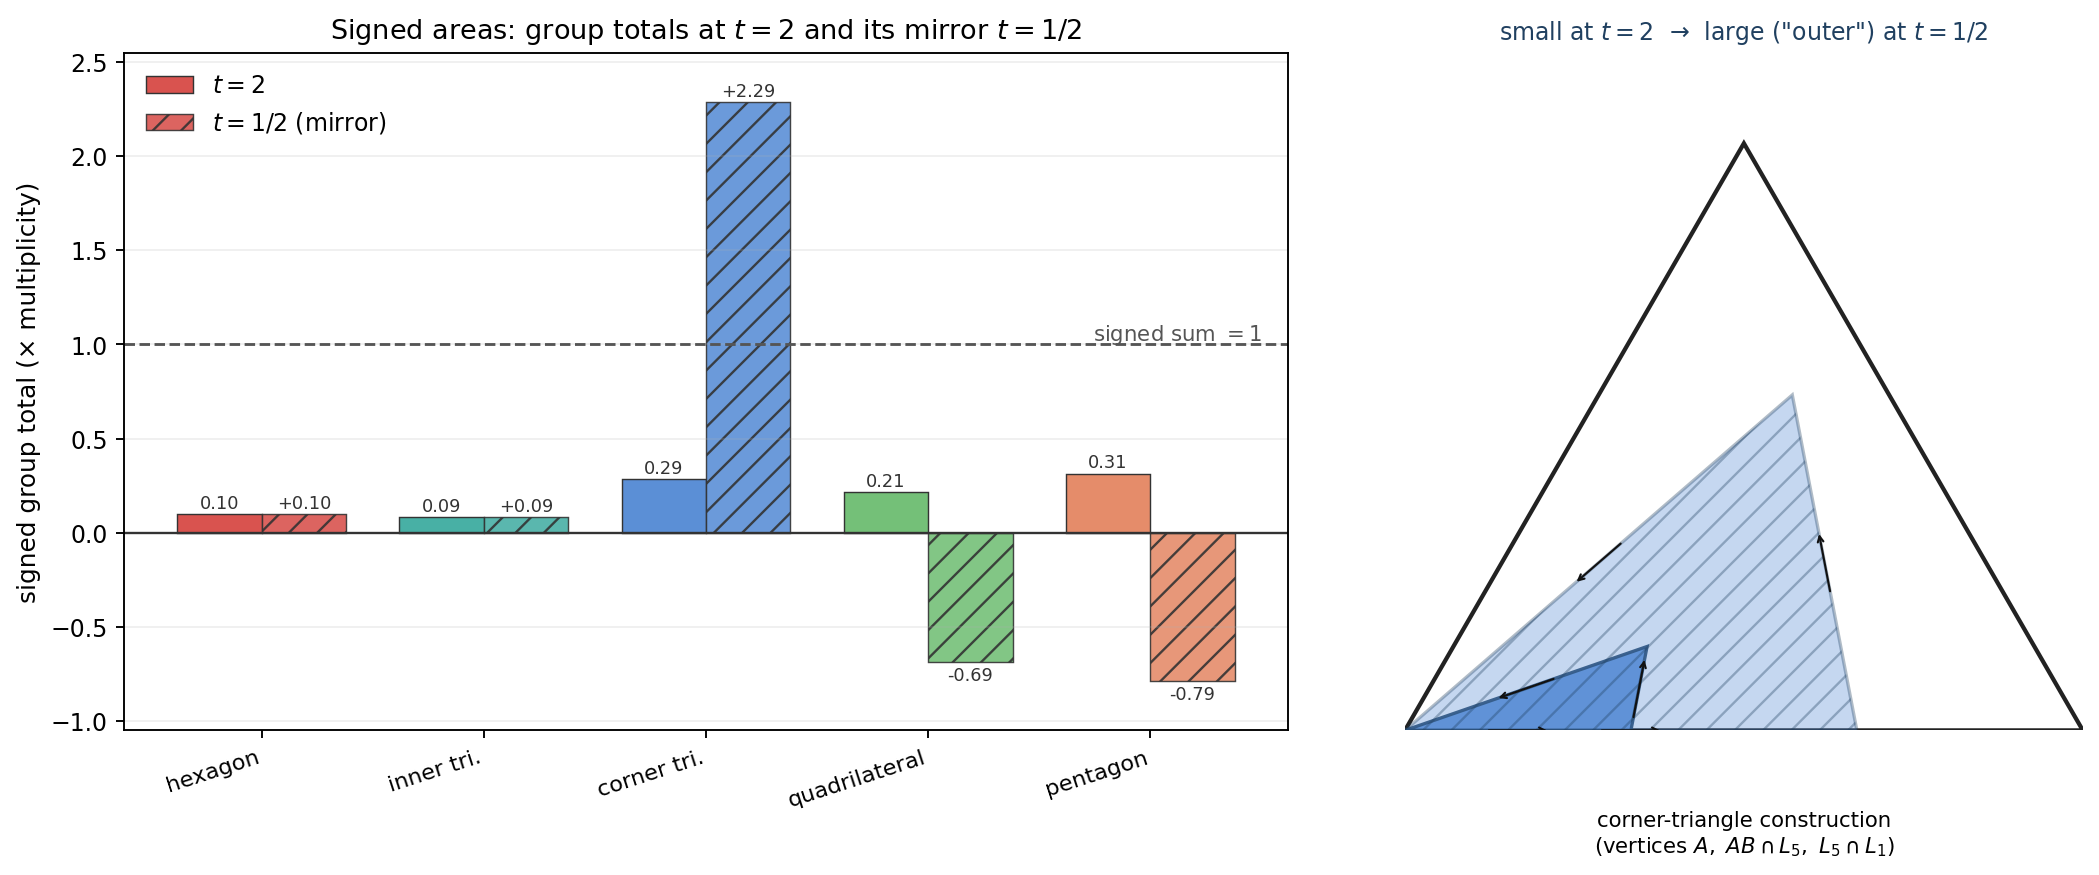
\includegraphics[width=\textwidth]{signed_cancellation.png}
\caption{Left: signed group totals at $t=2$ (all positive, summing to $1$) and at the mirror $t=1/2$ (the corner
triangles balloon to $+\tfrac{16}{7}$, the quadrilaterals and pentagons go negative), the signed sum staying $1$.
Right: the corner--triangle construction is a small interior cell at $t=2$ but a large outer triangle at $t=1/2$;
counter-clockwise arrows mark the orientation.}
\label{fig:signed}
\end{figure}

\begin{figure}[H]
\centering
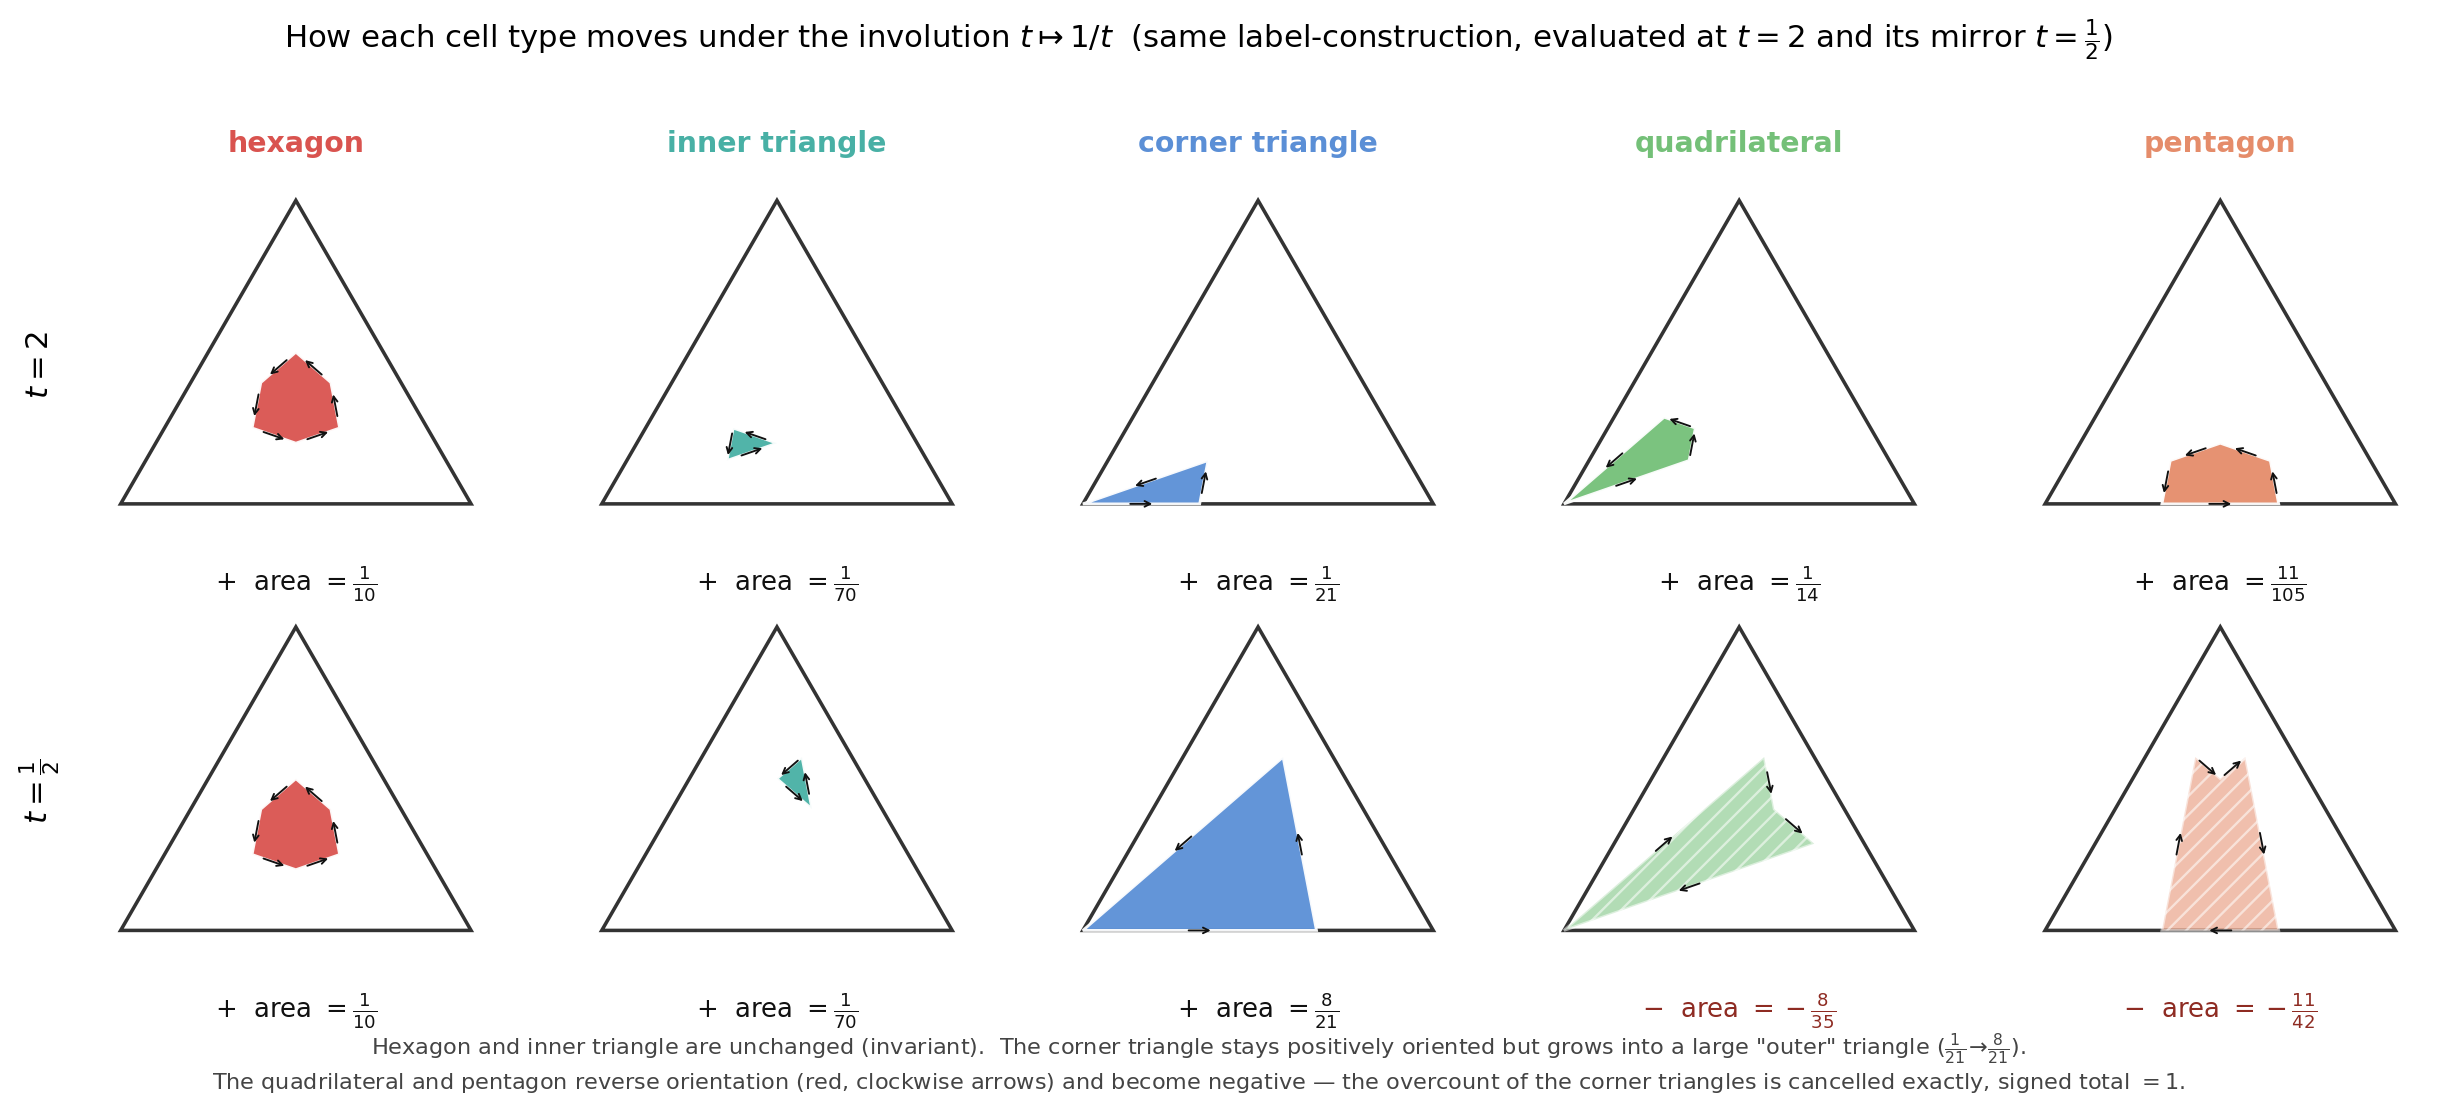
\includegraphics[width=\textwidth]{involution_by_type.png}
\caption{Every cell type under the involution: the same label-construction, evaluated at $t=2$ (top) and its
mirror $t=1/2$ (bottom), with counter-clockwise ($+$) or clockwise ($-$) boundary arrows. The hexagon and inner
triangle are unchanged (invariant, $B\equiv0$). The corner triangle keeps its positive orientation but swells from
$\tfrac1{21}$ to $\tfrac{8}{21}$ --- the ``outer'' triangle. The quadrilateral and pentagon reverse orientation
(red arrows) and turn negative; their new negative contributions cancel the corner triangles' overcount, and the
signed total stays $1$.}
\label{fig:move}
\end{figure}

\subsection{The quotient $\PP^1_u$ and the invariant/sign split}
Since the geometry depends only on $t$ modulo $\iota:t\mapsto1/t$, the true moduli space is the quotient
\[
\PP^1_t\big/\langle\iota\rangle\;\cong\;\PP^1_u,\qquad u=t+\tfrac1t,
\]
a degree--$2$ cover branched at the two fixed points $t=\pm1$ (that is $u=\pm2$); $t=0$ and $t=\infty$ both lie
over $u=\infty$. The branch point $t=1$ is precisely the median degeneration: the ramification of the cover
coincides with the geometric collapse.

Writing $w=t-\tfrac1t$, so that $w^2=u^2-4$ and $t=\tfrac{u+w}{2}$, each area splits uniquely into a part fixed by
$\iota$ (the trivial character of the deck group $\ZZ/2$) and a part changing sign (the sign character):
\[
\text{cell}=A(u)+B(u)\,w,\qquad w=\sqrt{u^2-4}.
\]
\begin{center}
\renewcommand{\arraystretch}{1.9}
\begin{tabular}{lcc}
\toprule
cell & $A(u)$ (invariant) & $B(u)$ (sign part) \\
\midrule
hexagon      & $\dfrac{2(u-2)}{2u+5}$ & $0$ \\
inner tri.   & $\dfrac{u-2}{(u+1)(2u+5)}$ & $0$ \\
corner tri.  & $\dfrac{u-1}{2(u+1)}$ & $-\dfrac{1}{2(u+2)}$ \\
quadrilateral& $\dfrac{(2-u)(u+3)}{(u+1)(2u+5)}$ & $\dfrac{1}{2u+5}$ \\
pentagon     & $\dfrac{(2-u)(u+3)}{(u+1)(2u+5)}$ & $\dfrac{u+3}{(u+2)(2u+5)}$ \\
\bottomrule
\end{tabular}
\end{center}
Three facts: the hexagon and inner triangle have $B\equiv0$ --- they descend to Möbius functions of $u$ on the base
$\PP^1_u$, whereas the other three genuinely require $\sqrt{u^2-4}$ and live on the double cover; the
quadrilateral and pentagon share the \emph{same} invariant part $A(u)$, differing only in their sign part; and at
the branch point $w=0$ ($u=2$, $t=1$) every cell collapses to its $A(u)$, giving $0$ for all but the corner, which
gives $A(2)=\tfrac16$ --- exactly the six medians. The decomposition already contains the median degeneration.

\section*{Glossary}
\begin{description}[leftmargin=0em,labelsep=0.5em,itemsep=2pt]
\item[Cevian] A segment from a vertex of a triangle to a point on the opposite side.
\item[Barycentric coordinates] Coordinates $(x:y:z)$ writing a point as $xA+yB+zC$ with $x+y+z=1$; vertices and
sides get the simple forms above, and (Lemma~\ref{lem:area}) triangle areas are $3\times3$ determinants.
\item[Affine map / affine invariance] A linear map followed by a translation. Affine maps carry any triangle to
any other and preserve ratios of areas; hence all area ratios here are shape--independent.
\item[Signed area / orientation (Umlaufrichtung)] The area of a polygon carries a sign fixed by the direction its
boundary is traversed: $+$ for counter-clockwise, $-$ for clockwise. The determinant of Lemma~\ref{lem:area} is a
signed area.
\item[CW--complex] A space assembled from cells of dimensions $0$ (points), $1$ (edges) and $2$ (regions); here,
the subdivision of the triangle by the nine lines.
\item[Chain; boundary operator $\partial$] A $k$--chain is a formal linear combination of oriented $k$--cells;
$\partial$ sends a cell to the signed sum of the cells on its boundary (a polygon to its edge cycle).
\item[Cochain; coboundary $\delta$] A $k$--cochain is a linear functional on $k$--chains --- a rule attaching a
number to each oriented $k$--cell (a $1$--cochain to edges, a $2$--cochain to cells). The coboundary
$\delta\varphi$ is defined by $(\delta\varphi)(\sigma)=\varphi(\partial\sigma)$: to evaluate it on a cell, sum
$\varphi$ around that cell's boundary. Here the area $2$--cochain equals $\delta\alpha$ for the edge cochain
$\alpha([P,Q])=[O,P,Q]$.
\item[Shoelace formula / discrete Stokes] The formula giving a polygon's area from its vertices; it is the
statement $\mathcal A=\delta\alpha$, the discrete case of Stokes' theorem.
\item[Ceva's theorem] Three cevians (one per vertex) are concurrent iff the product of the three side--division
ratios is $1$. ``Concurrent'' means passing through one common point.
\item[General position] No three lines through a common point --- the generic, non-degenerate situation.
\item[Group; $\ZZ/2$; involution] A group is a set with an associative product, identity and inverses. $\ZZ/2$ is
the two--element group; an \emph{involution} is an element (or map) equal to its own inverse, here
$\iota:t\mapsto1/t$.
\item[Group action] A rule by which each group element permutes the points of a set, compatibly with the group
product; here $\ZZ/2$ acts on the cells of each type by the foot--swap.
\item[Projective line $\PP^1$] The ordinary line plus one point ``at infinity''; the natural domain of a rational
function, on which $t=\infty$ is an honest point.
\item[Morphism] A structure--preserving map; for us a rational map $\PP^1\to\PP^1$.
\item[Covering (covering space); degree; sheets] A map $E\to X$ that locally looks like several disjoint copies
(``sheets'') of $X$; a degree--$d$ cover has $d$ sheets. Here $\PP^1_t\to\PP^1_u$, $u=t+1/t$, is a double cover:
a generic $u$ has the two preimages $t,1/t$.
\item[Branched (ramified) cover; branch point; ramification] A cover that is $d$--to--$1$ except over finitely
many \emph{branch points}, where sheets come together. Here the sheets $t,1/t$ coincide at $t=\pm1$ ($u=\pm2$),
the branch points; $t=1$ is simultaneously the median degeneration.
\item[Deck group / Galois group of a cover] The symmetries of a cover fixing the base. For $\PP^1_t\to\PP^1_u$ it
is $\ZZ/2=\langle\iota\rangle$, exchanging the two sheets. Degree--$2$ covers are automatically Galois (regular).
\item[Quotient $\PP^1_t/\langle\iota\rangle$] The space obtained by identifying $t$ with $1/t$; for this
involution it is again a projective line, coordinate $u=t+1/t$.
\item[Invariant / anti-invariant; trivial and sign characters] Under a $\ZZ/2$ action a function splits into an
even part fixed by the group (trivial character) and an odd part that changes sign (sign character). Here
``$A(u)+B(u)\sqrt{u^2-4}$'' is this splitting.
\item[Möbius function] A rational function $(au+b)/(cu+d)$; the hexagon area is one such function of $u$.
\end{description}

\end{document}
